\section{Security}

The authorization of JPM is implemented in the \security service. The \security
service provides two different services, which work together to form the
\security service:

\begin{enumerate}

    \item \textbf{An authentication system:} Responsible for proving identity
        of users.

    \item \textbf{An authorization system:} Responsible for deciding which
        users are allowed to do what.

\end{enumerate}

In this section, the client represents a service which uses the \security
services. The system is written to assume that a client \emph{is not} an actual
user. As a result most operations have been written to support various options
which should not be available to actual users. This means that when the
\security service is deployed, care must be taken to ensure that it is not
reachable by any ordinary user. Only the services which use the \security
service should be able to reach it. The services that use the \security
service, will then proxy only the relevant parts along.

\subsection{Authentication}
\label{sec:authentication}

The authentication system has a user based system. Users authenticate
themselves using a password. A group is a collection of users, which have an
associated set of permission. A single user may be part of many groups, it is
from groups that a user gains permission to use parts of the system. We cover
user permissions in Section \ref{sec:authorization}.

The authentication system is build following recommendations from
OWASP\autocite{OWASP1,OWASP2,OWASP3}. In this section the
authentication implementation, and rules surrounding the system are summarized.

\subsubsection*{Username and Password Rules}

The usernames used for the system are unique and case in-sensitive. The
username is required to be between 1 and 64 characters long. All character
types are allowed in usernames. Encoding of the usernames (and passwords) are
deployment dependent, specifically it depends on the protocol and its
configuration.

Passwords are case sensitive. The only limitation put on password is a length
requirement between 5 and 128 characters.

The maximum lengths used for these are mostly to establish reasonable limits.
Accepting an unlimited amount of data can be of concern for both storage and
amount of network traffic. For data that should be presented, i.e. username,
having a maximum is helpful for the design of user interfaces.

\subsubsection*{Storage}

The usernames and passwords are stored in a SQL database. The database itself,
along with its driver is configurable via the configuration system (See
Section \ref{sec:col}). Passwords are hashed with
BCrypt\footnote{BCrypt is a password hashing algorithm which has been used
by OpenBSD and others}\cite{provos1999future}, each individual password has
its own salt. ``Salting'' a password is the act of adding a randomly
generated string to each password. The salt itself isn't secret,
but is instead used to avoid precomputed reverse lookup tables for
the hashes (rainbow tables).

\subsubsection*{Authentication Process}

We start the discussion of how the authentication process works by looking at
how a client will successfully authenticate itself, this is shown in Figure
\ref{fig:auth_process}.

During the initial request nothing special really happens. The \security
service collaborates with both the \bcrypt service, along with its own
database. The database contains both \txtl{user} objects and \txtl{session}
objects. The \txtl{user} object has already been explained, and simply contains
the username, the hash of the salted password, and the salt itself. The
\txtl{session} object represents an active session. It contains the actual
token, which is a string generated by a cryptographically secure random number
generator. Along with this token, the object contains a timestamp for
generation, and a reference to the user object which created the session. The
timestamp will be used for implementing timeouts for the session.

At the end of the initial request, the client receives the token. This token is
what the client will have to provide for every privileged operation.  An
invalidation of a session may occur. This would ordinarily happen due to a
logout, or potentially a timeout which is handled by the client. The \security
service also supports checking the ``freshness'' of a session token, by making
sure it isn't older than some amount of time. This could be useful for ensuring
re-authentication before critical operations, such as changing your password.

\begin{figure}
    \begin{center}
    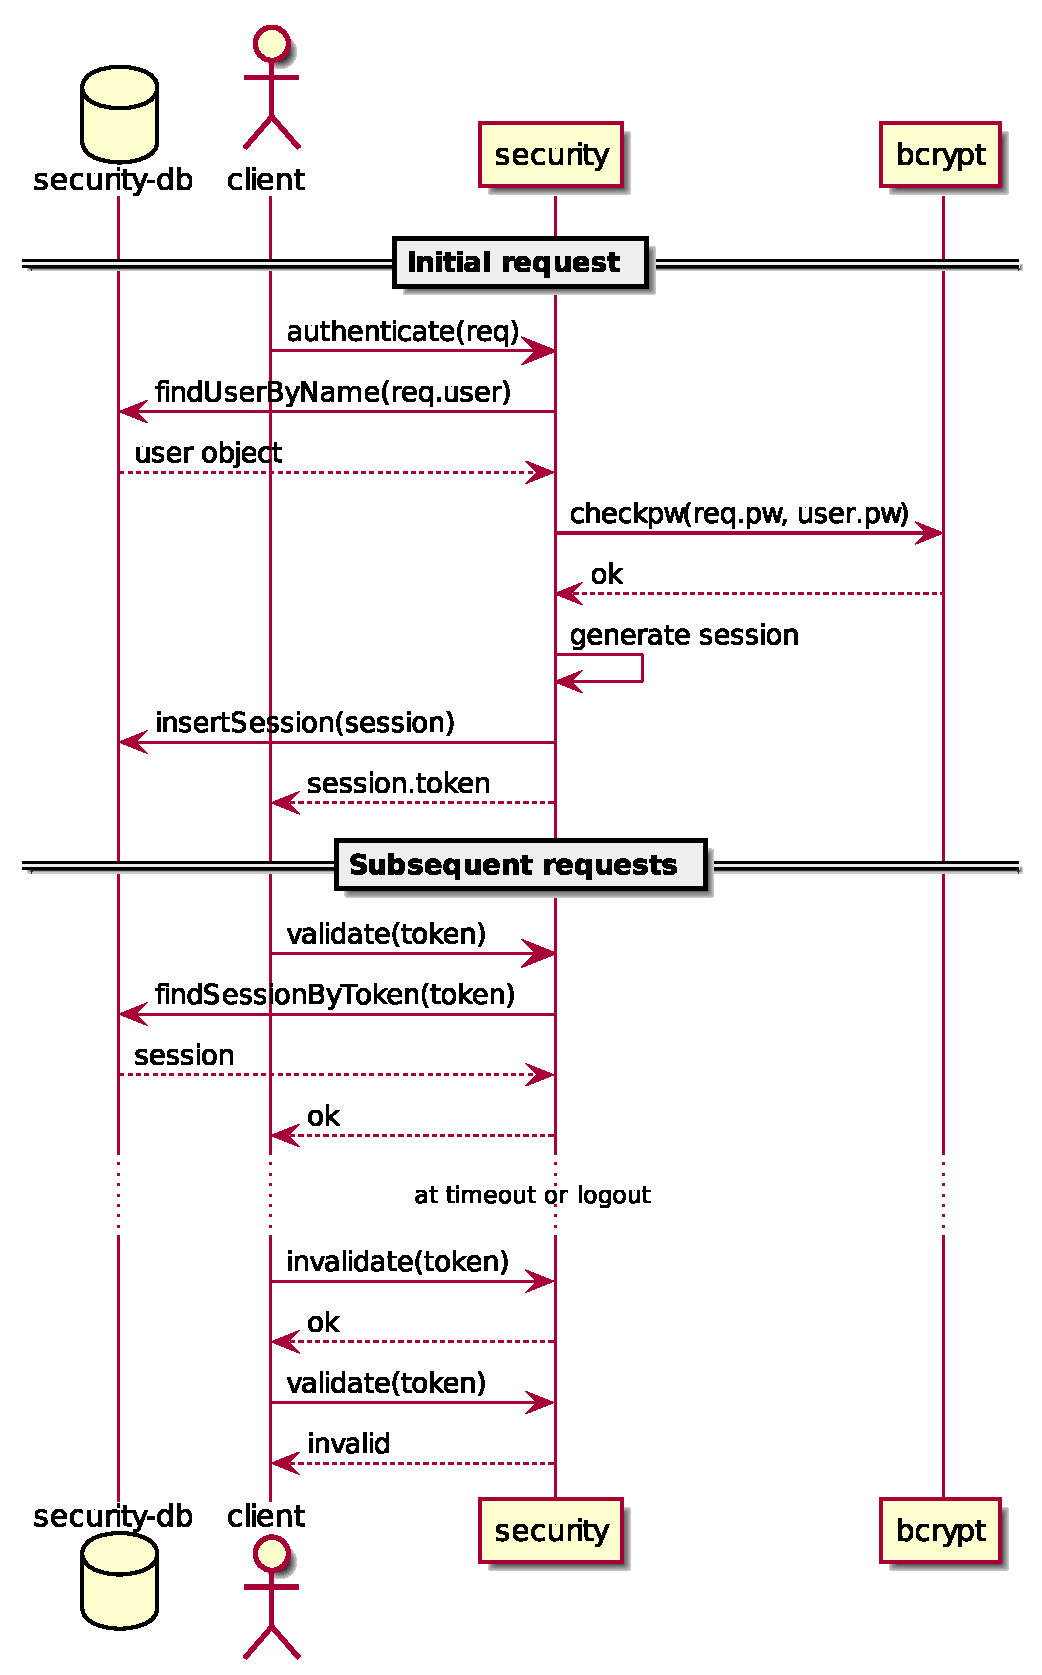
\includegraphics[width=0.8\textwidth]{package_manager/auth_sequence.eps}
    \end{center}
    \caption{The authentication process when successful}
    \label{fig:auth_process}
\end{figure}

Figure \ref{fig:auth_process} showed us the successful case. Internally,
validation will be performed at most steps. In the case of failure at
any of these steps a generic error message will be returned to the
client. The error message will only indicate if it was a user error or a
server error. This way an attacker cannot abuse the error messages for
information. For example given the error message ``Invalid password'' an
attacker would most likely be able to assume that the username itself is
correct.

\subsection{Authorization}
\label{sec:authorization}

% TODO More sources?
% https://en.wikipedia.org/wiki/Access_Control_Matrix#cite_ref-1

The authorization system based on an ``Access Control
Matrix''\cite{sandhu1994access} to define its security model. An access control
matrix, is a matrix $A$, where $A_{ij}$ contains the \emph{rights} that
\emph{role} $i$ has for \emph{resource} $j$.

A \emph{right} is a single piece of information. It describes something that an
entity is allowed to do for a specific resource in a role. In this
implementation a right is a simple string.

A \emph{resource} represents any entity that can have any rights associated
with it. This could, for example, be a file, which might have associated rights
such as ``read'' and ``write''.

A \emph{role} is some entity which have a set of rights for resources. In the
implementation roles have been replaced with \emph{groups}. A group is a
collection of users, which are provided by the authentication system.

Table \ref{tab:acm_example} shows an access control matrix for a few files,
which can be either read from or written to.

\begin{table}[H]
  \begin{center}
  \begin{tabular}{ | l | l | l | l | }
    \hline
            & \textbf{File 1}        & \textbf{File 2}      & \textbf{File 3}
    \\ \hline
    \textbf{Group 1} & read, write   & read                 &
    \\ \hline
    \textbf{Group 2} & read          & read                 & read, write
    \\ \hline
  \end{tabular}
  \end{center}

  \caption{A sample access control matrix for some computer files, which can be
      read from and written to by different groups}

  \label{tab:acm_example}
\end{table}

\subsection{Integration with JPM}

The \registry service is the only consumer of the \security service. On top of
this service the \registry service implements the security model JPM uses. JPM
supports users these map one-to-one with the user model of the \security
service. On top of this JPM supports teams which are supported by a single
underlying group. The purpose of a team is to allow for multiple users to all
have ownership of a single package. Every single user and team get their own
group, user groups only have a single member, while a team group has members
corresponding to the team. The user groups are named \txtl{users.<name>}, and
teams \txtl{groups.<name>}.

When a package is downloaded from or published to the \registry the user's
permissions will be checked. For a user to download a package, the user must be
in a group having the \txtl{read} (or \txtl{write} for publishing) right for
the corresponding resource. Each package has an associated resource called
\txtl{packages.<name>}. A wild card resource (\txtl{packages.*}) also exists.
The wild card resource represents every single package, thus if a group holds
the \txtl{packages.*/read} right then that group is allowed to download ever
package in the \registry. This is exactly how a \registry might provide guest
downloads.

TODO Find a place for this

Limiting number of login attempts within a period is often recommended. This is
done to avoid brute-force attacks. This isn't possible in Jolie, since the
sender isn't available to Jolie user code. This is most likely due to the fact
that no unique sender ID exists, since Jolie can accept messages from various
types of networks.
